\documentclass{article}
\usepackage{xcolor}
\usepackage{titleps}
\usepackage[letterpaper, margin=0.95in]{geometry}
\usepackage{url}
\usepackage{amsmath}
\usepackage{amssymb}
\usepackage{wrapfig}
\usepackage{float}
\usepackage{mathtools}
\usepackage{enumitem}
\usepackage{tabu}
\usepackage{parskip}
\usepackage{natbib}
\usepackage{listings}

\usepackage[many]{tcolorbox}
\usepackage{minted}
\setminted[python]{
	% frame=single,
	% linenos,
    xleftmargin=0.475em,
    baselinestretch=1.2,
}
% https://tex.stackexchange.com/a/569249
\setcounter{secnumdepth}{5}
\setcounter{tocdepth}{5}
\makeatletter
\newcommand\subsubsubsection{\@startsection{paragraph}{4}{\z@}{-2.5ex\@plus -1ex \@minus -.25ex}{1.25ex \@plus .25ex}{\normalfont\normalsize\bfseries}}
\newcommand\subsubsubsubsection{\@startsection{subparagraph}{5}{\z@}{-2.5ex\@plus -1ex \@minus -.25ex}{1.25ex \@plus .25ex}{\normalfont\normalsize\bfseries}}
\makeatother

\usepackage{hyperref}
\usepackage[color=red]{todonotes}
\usepackage{forest}
\definecolor{light-yellow}{HTML}{FFE5CC}

\newpagestyle{ruled}
{\sethead{CMU 16-831}{Introduction to Robot Learning }{Fall 2026}\headrule
  \setfoot{}{}{}}
\pagestyle{ruled}

\renewcommand\makeheadrule{\color{black}\rule[-.75\baselineskip]{\linewidth}{0.4pt}}
\renewcommand*\footnoterule{}

\newtcolorbox[]{answer}[1][]{
    % breakable,
    enhanced,
    nobeforeafter,
    colback=white,
    title=Your Answer,
    sidebyside align=top,
    box align=top,
    #1
}



\begin{document}

\lstset{basicstyle = \ttfamily,columns=fullflexible,
backgroundcolor = \color{light-yellow}
}

\begin{centering}
    {\Large Assignment 2: Policy Gradient} \\
    \vspace{.25cm}
    % \textbf{Due September 13, 11:59 pm} \\
\end{centering}
\vspace{0.25cm}

\textbf{Andrew ID:} \texttt{vawale} \\
\textbf{Collaborators:} \texttt{None. Claude (Anthropic) helped with the code and with formatting the text.}\\
\textbf{NOTE:} Please do \textbf{NOT} change the sizes of the answer blocks or plots.

\setcounter{section}{4}
\section{Small-Scale Experiments (7.5 Pts)}

\subsection{Experiment 1 (Cartpole) -- \lbrack4.5 points total\rbrack}

\subsubsection{Configurations}
\begin{answer}[title=Q5.1.1,height=6cm,width=\linewidth]
% TODO
\begin{minted}
[framesep=2mm, fontsize=\scriptsize, breaklines]
{bash}
python rob831/scripts/run_hw2.py --env_name CartPole-v0 -n 150 -b 1500 \
    -dsa --exp_name q1_sb_no_rtg_dsa

python rob831/scripts/run_hw2.py --env_name CartPole-v0 -n 150 -b 1500 \
    -rtg -dsa --exp_name q1_sb_rtg_dsa

python rob831/scripts/run_hw2.py --env_name CartPole-v0 -n 150 -b 1500 \
    -rtg --exp_name q1_sb_rtg_na

python rob831/scripts/run_hw2.py --env_name CartPole-v0 -n 150 -b 6000 \
    -dsa --exp_name q1_lb_no_rtg_dsa

python rob831/scripts/run_hw2.py --env_name CartPole-v0 -n 150 -b 6000 \
    -rtg -dsa --exp_name q1_lb_rtg_dsa

python rob831/scripts/run_hw2.py --env_name CartPole-v0 -n 150 -b 6000 \
    -rtg --exp_name q1_lb_rtg_na
\end{minted}
\end{answer}

\subsubsection{Plots}

\subsubsubsection{Small batch -- \lbrack1 points\rbrack}
\begin{answer}[title=Q5.1.2.1,height=9.5cm,width=\linewidth]
\centering
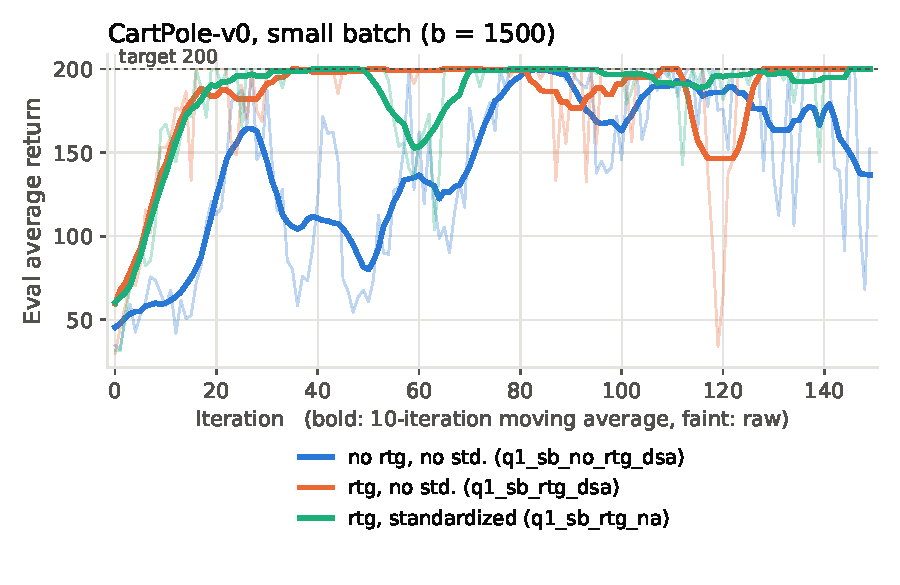
\includegraphics[height=8cm]{figures/q1_small_batch.pdf}
\end{answer}

\subsubsubsection{Large batch -- \lbrack0.5 points\rbrack}
\begin{answer}[title=Q5.1.2.2,height=9.5cm,width=\linewidth]
\centering
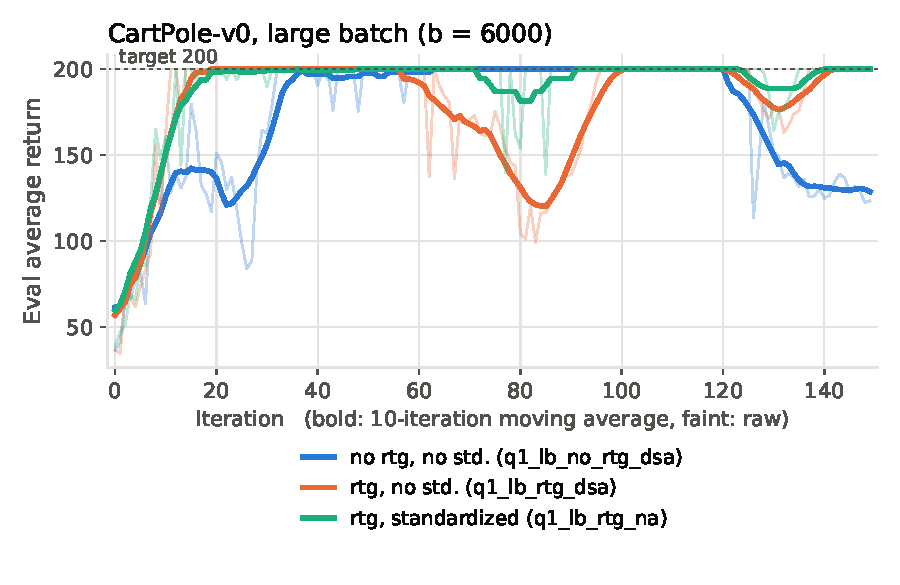
\includegraphics[height=8cm]{figures/q1_large_batch.pdf}
\end{answer}

\subsubsection{Analysis}

\subsubsubsection{Value estimator -- \lbrack1 points\rbrack}
\begin{answer}[title=Q5.1.3.1,height=4cm,width=\linewidth]
Reward-to-go is clearly better. Comparing the two runs without standardization, reward-to-go reached 200 about twice as fast (by iteration 16 instead of 27 with the small batch, and 11 instead of 32 with the large one) and then mostly stayed there, while the trajectory-centric estimator kept falling back and ended below 200 at both batch sizes. The reason is variance: the full-trajectory return credits every action with rewards that were earned before it was taken, which the action could not have influenced. Reward-to-go drops those terms, so each gradient estimate carries less noise and the policy improves more steadily.
\end{answer}

\subsubsubsection{Advantage standardization -- \lbrack1 points\rbrack}
\begin{answer}[title=Q5.1.3.2,height=4cm,width=\linewidth]
Yes, for stability rather than speed. The two reward-to-go runs reached 200 at essentially the same iteration with and without standardization. The difference came afterwards: without it, the small-batch run collapsed to a return of 34 after having solved the task, whereas with it the return never fell below about 100, and the large batch showed the same pattern. Standardizing keeps the size of each update roughly constant regardless of how large the raw returns are in that batch, so one batch of unusually long or short episodes cannot produce an oversized step that undoes earlier progress.
\end{answer}

\subsubsubsection{Batch size -- \lbrack1 points\rbrack}
\begin{answer}[title=Q5.1.3.3,height=4cm,width=\linewidth]
Yes. With the larger batch the reward-to-go runs reached 200 a few iterations sooner (around iteration 11 instead of 16) and, more noticeably, their dips after reaching 200 were much shallower. A batch of 6000 steps averages the gradient over roughly four times as many trajectories, so each update points more reliably in the right direction. The trajectory-centric estimator is the exception: even with the large batch it kept oscillating and finished below 200, so simply collecting more data did not compensate for the extra variance that estimator carries. Reward-to-go removes that variance at its source, which is why it benefits more from a larger batch.
\end{answer}

\subsection{Experiment 2 (InvertedPendulum) -- \lbrack3 points total\rbrack}

\subsubsection{Configurations -- \lbrack1 points\rbrack}
\begin{answer}[title=Q5.2.1,height=10cm,width=\linewidth]
\begin{minted}
[framesep=2mm, fontsize=\scriptsize, breaklines]
{bash}
# Best run (b* = 300, r* = 0.01):
python rob831/scripts/run_hw2.py --env_name InvertedPendulum-v4 \
    --ep_len 1000 --discount 0.92 -n 100 -l 2 -s 64 -b 300 -lr 0.01 -rtg \
    --seed 5 --exp_name q2_b300_r0.01

# Search: the same command for every pair of
#   <b> in {100, 200, 300, 500, 1000, 2000, 5000} and <r> in {0.005, 0.01, 0.02, 0.05}
python rob831/scripts/run_hw2.py --env_name InvertedPendulum-v4 \
    --ep_len 1000 --discount 0.92 -n 100 -l 2 -s 64 -b <b> -lr <r> -rtg \
    --seed 5 --exp_name q2_b<b>_r<r>
\end{minted}
\end{answer}

\subsubsection{smallest \textbf{b*} and largest \textbf{r*} (same run) -- \lbrack1 points\rbrack}
\begin{answer}[title=Q5.2.2,height=4cm,width=\linewidth]
$b^* = 300$, $r^* = 0.01$ (seed 5). I chose this as the smallest batch and largest learning rate at which the policy not only reaches 1000 but stays there: it first hits 1000 at iteration 57 and holds near 1000 for the last 15 iterations. Pushing further did not work. At the same batch size, $r=0.02$ never reached 1000, and $r=0.05$ did hit 1000 several times but kept collapsing to near zero in between, since a step that large keeps overshooting. Batches of 100 and 200 were too noisy at every learning rate: each touched 1000 only a handful of times and ended far below it.
\end{answer}

\subsubsection{Plot -- \lbrack1 points\rbrack}
\begin{answer}[title=Q5.2.3,height=10cm,width=\linewidth]
\centering
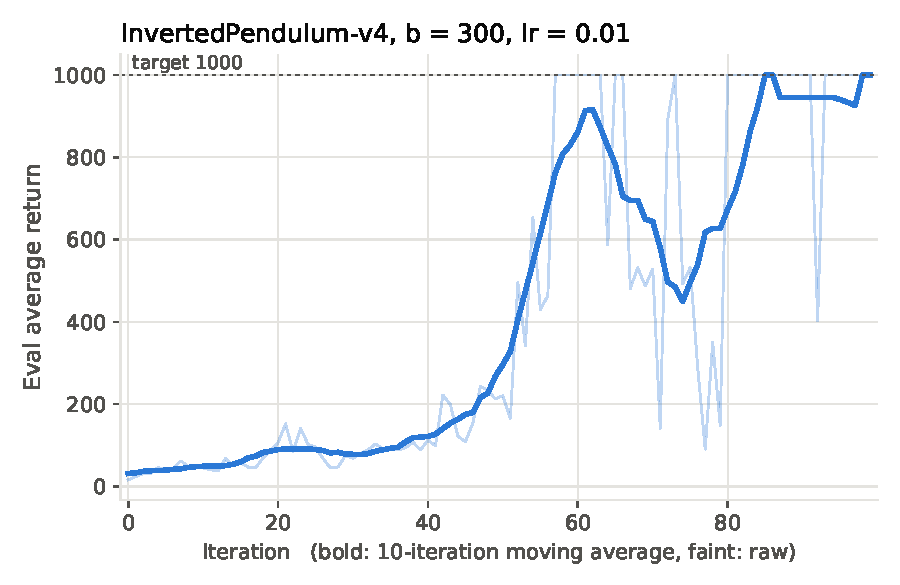
\includegraphics[height=8cm]{figures/q2_b300_r0_01.pdf}
\end{answer}

\setcounter{section}{6}
\section{More Complex Experiments (4.5 Pts)}

\subsection{Experiment 3 (LunarLander) -- \lbrack1 points total\rbrack}

\subsubsection{Configurations}
\begin{answer}[title=Q7.1.1,height=6cm,width=\linewidth]
\begin{minted}
[framesep=2mm, fontsize=\scriptsize, breaklines]
{bash}
python rob831/scripts/run_hw2.py \
    --env_name LunarLanderContinuous-v2 --ep_len 1000 \
    --discount 0.99 -n 100 -l 2 -s 64 -b 10000 -lr 0.005 \
    --reward_to_go --nn_baseline --exp_name q3_b10000_r0.005
\end{minted}
\end{answer}

\subsubsection{Plot -- \lbrack1 points\rbrack}
\begin{answer}[title=Q7.1.2,height=10cm,width=\linewidth]
\centering
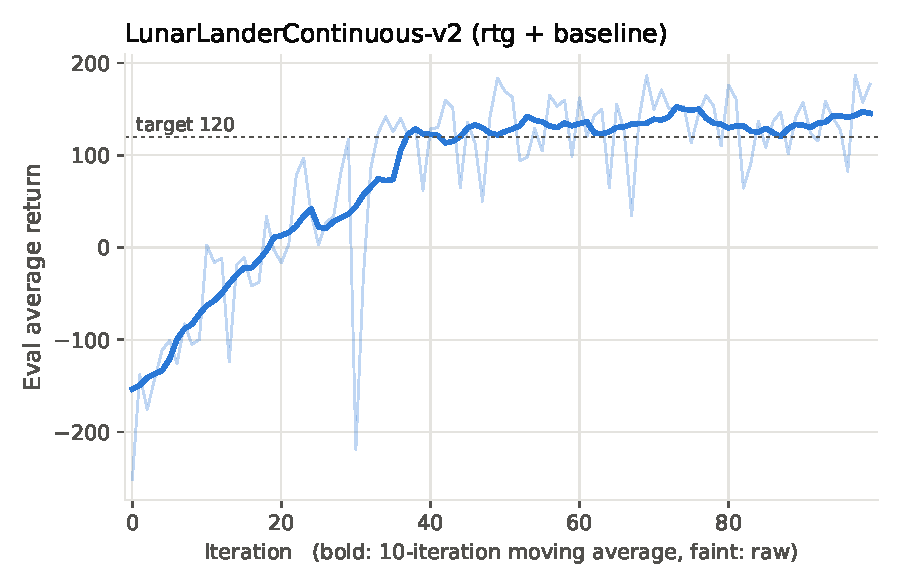
\includegraphics[height=8cm]{figures/q3_lunarlander.pdf}
\end{answer}

\subsection{Experiment 4 (HalfCheetah) -- \lbrack3.5 points\rbrack}

\subsubsection{Configurations}
\begin{answer}[title=Q7.2.1,height=10cm,width=\linewidth]
\begin{minted}
[framesep=2mm, fontsize=\scriptsize, breaklines, escapeinside=||, mathescape=true]
{python}
# Search (plotted in Q7.2.2): the same command for every pair of
#   <b> in {10000, 30000, 50000} and <r> in {0.005, 0.01, 0.02}
python rob831/scripts/run_hw2.py --env_name HalfCheetah-v4 --ep_len 150 \
    --discount 0.95 -n 100 -l 2 -s 32 -b <b> -lr <r> -rtg --nn_baseline \
    --seed 5 --exp_name q4_search_b<b>_lr<r>_rtg_nnbaseline

# Extra comparison at the smallest batch (plotted in Q7.2.4): the four
# estimator variants with b = 10000, lr = 0.02
python rob831/scripts/run_hw2.py --env_name HalfCheetah-v4 --ep_len 150 \
    --discount 0.95 -n 100 -l 2 -s 32 -b 10000 -lr 0.02 \
    --seed 5 --exp_name q4_b10000_r0.02
python rob831/scripts/run_hw2.py --env_name HalfCheetah-v4 --ep_len 150 \
    --discount 0.95 -n 100 -l 2 -s 32 -b 10000 -lr 0.02 -rtg \
    --seed 5 --exp_name q4_b10000_r0.02_rtg
python rob831/scripts/run_hw2.py --env_name HalfCheetah-v4 --ep_len 150 \
    --discount 0.95 -n 100 -l 2 -s 32 -b 10000 -lr 0.02 --nn_baseline \
    --seed 5 --exp_name q4_b10000_r0.02_nnbaseline
python rob831/scripts/run_hw2.py --env_name HalfCheetah-v4 --ep_len 150 \
    --discount 0.95 -n 100 -l 2 -s 32 -b 10000 -lr 0.02 -rtg --nn_baseline \
    --seed 5 --exp_name q4_b10000_r0.02_rtg_nnbaseline
\end{minted}
\end{answer}

\subsubsection{Plot -- \lbrack1 points\rbrack}
\begin{answer}[title=Q7.2.2,height=10cm,width=\linewidth]
\centering
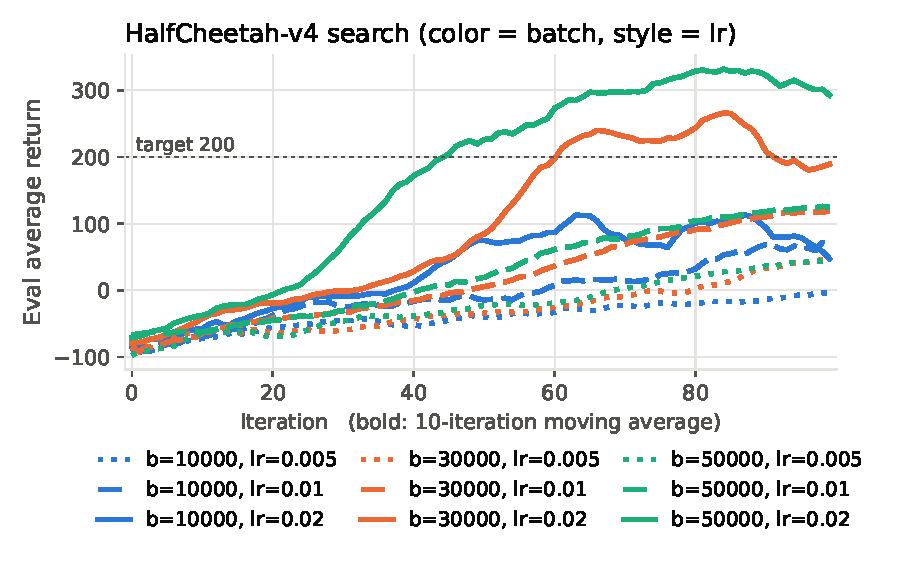
\includegraphics[height=8cm]{figures/q4_search.pdf}
\end{answer}

\subsubsection{ Optimal b* and r* -- \lbrack0.5 points\rbrack}
\begin{answer}[title=Q7.2.3,height=4cm,width=\linewidth]
$b^* = 50000$, $r^* = 0.02$ (seed 5). This setting had the highest return in the search: 344 at the final iteration, with an average of 310 over the last 10 iterations.
\end{answer}

\subsubsection{ Plot -- \lbrack0.5 points\rbrack}
\begin{answer}[title=Q7.2.4,height=10cm,width=\linewidth]
\centering
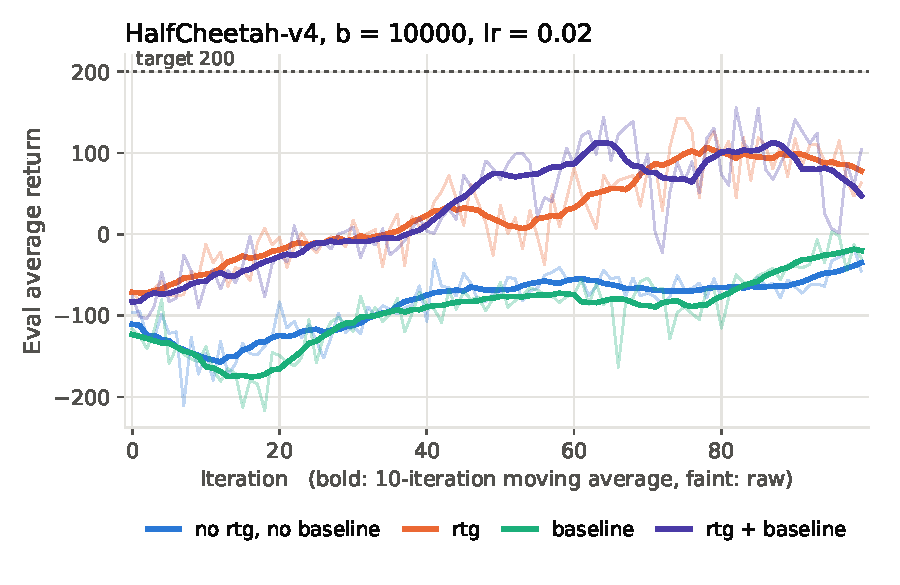
\includegraphics[height=8cm]{figures/q4_final_b10000_r0_02.pdf}
\end{answer}

\subsubsection{ Describe how b* and r* affect task performance -- \lbrack0.5 points\rbrack}
\begin{answer}[title=Q7.2.5,height=4cm,width=\linewidth]
The learning rate mattered most: at every batch size the final return rose with it, and the largest value, 0.02, was best everywhere, since with only 100 iterations the smaller steps do not get far (at $b=50000$ the final return went from 46 to 344 between 0.005 and 0.02). Batch size mattered mainly once the step was large: at 0.02 the final return roughly tripled from $b=10000$ to 50000, because the large batch averages out gradient noise and lets the big step be taken without the drops the 10000-step runs show. A large step is only safe when the gradient is good enough to trust. The baseline also helped more at the large batch (Q7.2.7 vs.\ Q7.2.4), though with one seed I cannot rule out noise.
\end{answer}

\subsubsection{Configurations with optimal b* and r* -- \lbrack0.5 points\rbrack}
\begin{answer}[title=Q7.2.6,height=6cm,width=\linewidth]
\begin{minted}
[framesep=2mm, fontsize=\scriptsize, breaklines]
{bash}
python rob831/scripts/run_hw2.py --env_name HalfCheetah-v4 --ep_len 150 \
    --discount 0.95 -n 100 -l 2 -s 32 -b 50000 -lr 0.02 \
    --seed 5 --exp_name q4_b50000_r0.02

python rob831/scripts/run_hw2.py --env_name HalfCheetah-v4 --ep_len 150 \
    --discount 0.95 -n 100 -l 2 -s 32 -b 50000 -lr 0.02 -rtg \
    --seed 5 --exp_name q4_b50000_r0.02_rtg

python rob831/scripts/run_hw2.py --env_name HalfCheetah-v4 --ep_len 150 \
    --discount 0.95 -n 100 -l 2 -s 32 -b 50000 -lr 0.02 --nn_baseline \
    --seed 5 --exp_name q4_b50000_r0.02_nnbaseline

python rob831/scripts/run_hw2.py --env_name HalfCheetah-v4 --ep_len 150 \
    --discount 0.95 -n 100 -l 2 -s 32 -b 50000 -lr 0.02 -rtg --nn_baseline \
    --seed 5 --exp_name q4_b50000_r0.02_rtg_nnbaseline
\end{minted}
\end{answer}

\subsubsection{Plot for four runs with optimal b* and r* -- \lbrack0.5 points\rbrack}
\begin{answer}[title=Q7.2.7,height=10cm,width=\linewidth]
\centering
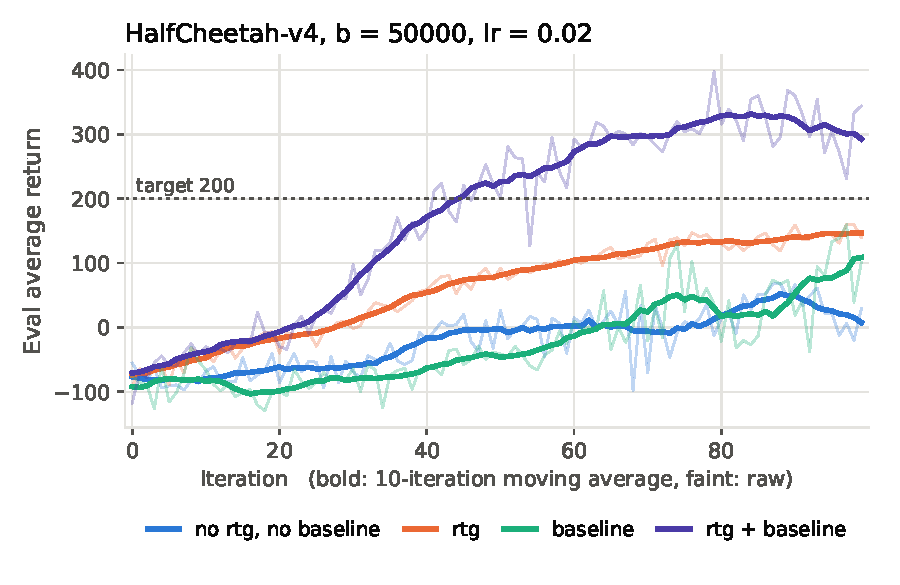
\includegraphics[height=8cm]{figures/q4_final_b50000_r0_02.pdf}
\end{answer}

\section{Implementing Generalized Advantage Estimation (3 Pts)}

\subsection{Experiment 5 (Hopper) -- \lbrack3 points\rbrack}

\subsubsection{Configurations}
\begin{answer}[title=Q8.1.1,height=4cm,width=\linewidth]
\begin{minted}
[framesep=2mm, fontsize=\scriptsize, breaklines, escapeinside=||, mathescape=true]
{python}
# $\lambda \in [0,0.95,0.99,1]$
python rob831/scripts/run_hw2.py \
    --env_name Hopper-v4 --ep_len 1000 \
    --discount 0.99 -n 300 -l 2 -s 32 -b 2000 -lr 0.001 \
    --reward_to_go --nn_baseline --action_noise_std 0.5 --gae_lambda <|$\lambda$|> \
    --exp_name q5_b2000_r0.001_lambda<|$\lambda$|>
\end{minted}
\end{answer}

\subsubsection{Plot -- \lbrack1 points\rbrack}
\begin{answer}[title=Q8.1.2,height=10cm,width=\linewidth]
\centering
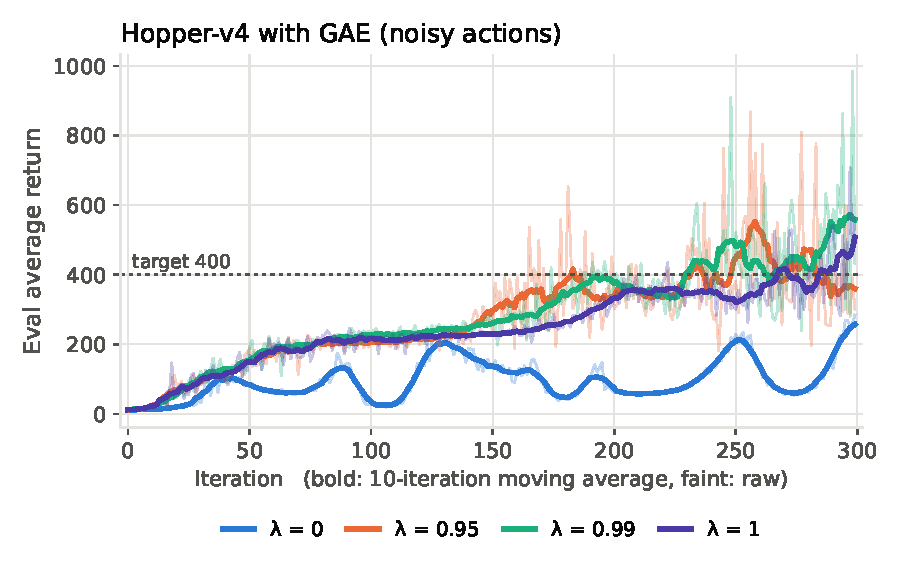
\includegraphics[height=8cm]{figures/q5_hopper.pdf}
\end{answer}

\subsubsection{Describe how $\lambda$ affects task performance -- \lbrack1.5 points\rbrack}
\begin{answer}[title=Q8.1.3,height=4cm,width=\linewidth]
$\lambda$ sets how much the advantage estimate trusts the learned value function versus observed rewards, and the results follow the expected bias--variance trade-off. With $\lambda=0$ the advantage is the one-step TD error, so it leans entirely on a still-inaccurate value function: this run never reached 400 and kept oscillating. Raising $\lambda$ mixes in longer stretches of real rewards, removing that bias at the cost of noisier estimates: $\lambda=0.95$, 0.99 and 1 all passed 400, with 0.99 best overall (about 460 over the last 50 iterations). $\lambda=1$, the plain Monte Carlo baseline estimator, was slowest to get going because of its higher variance, though it ended highest at 564.
\end{answer}

\subsubsection{Find one robotics paper from the last 5 years that uses policy gradients or an actor-critic method as part of its methodology. 
    In a short paragraph (4--5 sentences): (i) cite the paper, (ii) briefly describe the robot task and how reinforcement learning is used, and (iii) identify one technique from this homework (e.g., reward-to-go, a value-function baseline, or GAE) that is related to the method used in the paper. A few sentences is enough; this is not meant to be an extensive literature review  -- \lbrack0.5 points\rbrack
}
\begin{answer}[title=Q8.1.4,height=4cm,width=\linewidth]
E.~Kaufmann, L.~Bauersfeld, A.~Loquercio, M.~M\"uller, V.~Koltun and D.~Scaramuzza, ``Champion-level drone racing using deep reinforcement learning,'' \emph{Nature} 620, 982--987 (2023). Their system, Swift, races a quadrotor through a gate course against human world champions using only onboard sensing. The control policy maps the estimated drone state to thrust and body-rate commands and is trained in simulation with PPO, an on-policy actor-critic policy-gradient method. PPO's critic is a learned value function subtracted from the return to form the advantage, which is the value-function baseline used in this homework.
\end{answer}

\end{document}
